\documentclass[11pt,a4paper]{article}

\usepackage[margin=24mm]{geometry}
\usepackage[T1]{fontenc}
\usepackage[utf8]{inputenc}
\usepackage{lmodern}
\usepackage{microtype}
\usepackage{amsmath,amssymb,bm}
\usepackage{booktabs,longtable,array}
\usepackage{graphicx}
\usepackage{xcolor}
\usepackage{hyperref}
\usepackage{listings}
\usepackage{tikz}
\usepackage{pgfplots}
\usetikzlibrary{arrows.meta,calc,positioning,fit,backgrounds,decorations.pathmorphing}
\pgfplotsset{compat=1.18}

\hypersetup{
  colorlinks=true,
  linkcolor=blue!55!black,
  urlcolor=blue!55!black,
  citecolor=blue!55!black,
  pdftitle={Manual for urdf_to_standard_dh.py},
  pdfauthor={ChatGPT generated manual}
}

\definecolor{codebg}{RGB}{248,248,248}
\definecolor{codeframe}{RGB}{210,210,210}
\definecolor{darkgreen}{RGB}{0,100,0}

\lstdefinestyle{manualcode}{
  basicstyle=\ttfamily\small,
  backgroundcolor=\color{codebg},
  frame=single,
  rulecolor=\color{codeframe},
  breaklines=true,
  columns=fullflexible,
  keepspaces=true,
  showstringspaces=false,
  keywordstyle=\color{blue!60!black},
  commentstyle=\color{darkgreen},
  stringstyle=\color{orange!60!black}
}
\lstset{style=manualcode}

\newcommand{\R}{\mathbb{R}}
\newcommand{\T}{\mathbf{T}}
\newcommand{\Rot}{\operatorname{Rot}}
\newcommand{\Trans}{\operatorname{Trans}}
\newcommand{\atan}{\operatorname{atan2}}
\newcommand{\norm}[1]{\left\lVert #1 \right\rVert}
\newcommand{\codepath}[1]{\path{#1}}

\title{Manual for \path{urdf_to_standard_dh.py}\\[2mm]
\large Generation of a PSDM-compatible standard DH table from one serial URDF chain}
\author{Generated for the Robot System Identification workflow}
\date{\today}

\begin{document}
\maketitle

\begin{abstract}
This manual documents the Python script \path{urdf_to_standard_dh.py}. The script parses one serial chain from a URDF file, constructs a candidate standard Denavit-Hartenberg (DH) representation, writes the PSDM-compatible DH matrix, and verifies the result by forward-kinematics comparison. The manual describes the command-line interface, the expected YAML configuration, the generated outputs, the mathematical construction implemented by the script, and its limitations. The script intentionally keeps actuator-side encoder conversion, gearbox ratios, ball-screw conversion, and current-to-effort conversion outside the kinematic DH generation step.
\end{abstract}

\tableofcontents
\newpage

\section{Purpose and scope}

The script generates a standard DH table compatible with the PSDM MATLAB package. The generated numeric table has one row per active joint and six columns:
\begin{equation}
  \mathrm{DH}_i = \begin{bmatrix} a_i & \alpha_i & d_i & \theta_i & t_i & s_i \end{bmatrix}.
\end{equation}
Here $t_i = 0$ denotes a revolute joint, $t_i = 1$ denotes a prismatic joint, and $s_i$ is the PSDM joint sign. Under the implemented policy, the PSDM coordinate is the URDF joint coordinate:
\begin{equation}
  q_{\mathrm{PSDM},i} = q_{\mathrm{URDF},i}.
\end{equation}
Therefore the generated sign column is $s_i = +1$ for all active joints. The sign and scale from motor encoder counts to physical joint coordinates remain separate preprocessing data and are not embedded in the DH table.

\subsection{Implemented behavior}

The script performs the following operations:
\begin{enumerate}
  \item Reads the YAML configuration.
  \item Parses the URDF XML joint tree.
  \item Extracts the parent chain from the configured base link to the configured tool link.
  \item Folds fixed joints into the geometric transform chain.
  \item Treats continuous joints as revolute joints.
  \item Builds DH frames from the active joint axes at $q=0$.
  \item Extracts standard DH parameters from the relative frame transforms.
  \item Writes CSV, optional MAT, JSON, Markdown reports, and a convention-sheet draft.
  \item Validates the result by comparing URDF forward kinematics and DH forward kinematics on random joint samples.
\end{enumerate}

\subsection{Deliberate exclusions}

The script does not solve the complete system-identification data-conversion problem. It does not process motor encoder counts, gear ratios, ball-screw leads, drive signs, current signs, or current-to-effort constants. Those quantities belong to the actuator-to-joint preprocessing stage and to the torque or generalized-effort measurement model.

The script also does not attempt to support every possible URDF topology. It is intentionally limited to one selected serial chain. Mimic joints are rejected. Non-serial branches outside the selected chain are ignored.

\section{Input files and command line}

\subsection{Command line}

The normal invocation is:
\begin{lstlisting}[language=bash]
python3 urdf_to_standard_dh.py \
  --config urdfToDhTemplate.yaml \
  --output-dir urdf_to_dh_output
\end{lstlisting}

The URDF file can be overridden from the command line:
\begin{lstlisting}[language=bash]
python3 urdf_to_standard_dh.py \
  --config urdfToDhTemplate.yaml \
  --urdf another_robot.urdf \
  --output-dir urdf_to_dh_output
\end{lstlisting}

\subsection{Dependencies}

The required dependencies are:
\begin{lstlisting}[language=bash]
python3 -m pip install numpy pyyaml
\end{lstlisting}

The optional MAT-file output requires SciPy:
\begin{lstlisting}[language=bash]
python3 -m pip install scipy
\end{lstlisting}

The script uses only standard Python XML parsing plus NumPy. It does not require a ROS installation.

\subsection{Configuration file}

The relevant configuration fields are:
\begin{lstlisting}[language={}]
urdf:
  upload: "urdf_eb1.1.xml"
  base_link: "starman_arm_link_cart"
  tool_link: "starman_arm_ids"

coordinate_policy:
  dh_q_reference: "URDF joint coordinate at q = 0"
  joint_sign_policy: "URDF_coordinate"
  emit_residual_transforms: true

fk_validation:
  random_samples: 100
  position_tolerance_m: 0.001
  orientation_tolerance_deg: 0.1
  continuous_joint_sampling_range_rad: [-3.141592653589793, 3.141592653589793]
\end{lstlisting}

Only the two coordinate-policy values shown above are currently implemented. This restriction is intentional. Encoder offsets and drive signs should not be mixed into the purely geometric URDF-to-DH conversion.

\section{Generated outputs}

For the configured sample, the script writes the following files into the output directory.

\begin{longtable}{@{}p{0.32\linewidth}p{0.60\linewidth}@{}}
\toprule
File & Purpose \\
\midrule
\path{dh_table.csv} & Human-readable PSDM DH table, including joint names and columns $[a,\alpha,d,\theta,t,s]$. \\
\path{dh_table.mat} & MATLAB file containing variable \texttt{DH} and the joint-name list. Written only if SciPy is installed and enabled. \\
\path{urdf_kinematics.json} & Joint order, generated DH matrix, active joint axes at $q=0$, and residual transforms. \\
\path{dh_mapping_report.md} & Markdown report containing the generated DH table, residual transforms, and RPY normalization notes. \\
\path{conventions_sheet.draft.md} & Draft joint-convention table, including local and base-frame positive joint axes at $q=0$. \\
\path{fk_validation_report.md} & Random-sample FK validation status and maximum errors. \\
\bottomrule
\end{longtable}

\section{Coordinate conventions}

\subsection{URDF transform convention}

For each URDF joint, the script uses the joint origin transform first, followed by joint motion. For a chain of joints $j=1,\ldots,m$, the URDF forward kinematics are:
\begin{equation}
  \T_{\mathrm{URDF}}(q) = \prod_{j=1}^{m} \T_{\mathrm{origin},j}\,\T_{\mathrm{motion},j}(q_j),
\end{equation}
where fixed joints have $\T_{\mathrm{motion},j}=I$ and active joints contribute either a revolute or prismatic motion.

\begin{figure}[htbp]
\centering
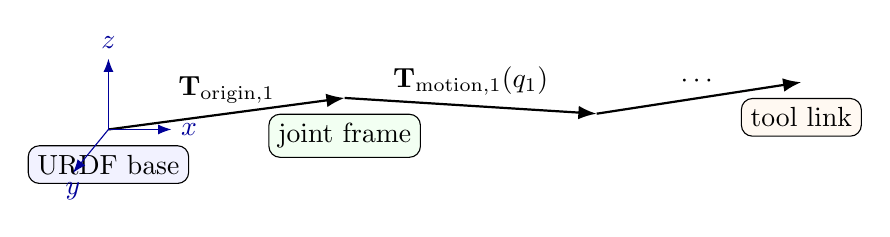
\begin{tikzpicture}[>=Latex, scale=1.0]
  \coordinate (B) at (0,0);
  \coordinate (O1) at (3.0,0.4);
  \coordinate (O2) at (6.2,0.2);
  \coordinate (T) at (8.8,0.6);
  \draw[->, thick] (B) -- (O1) node[midway, above] {$\T_{\mathrm{origin},1}$};
  \draw[->, thick] (O1) -- (O2) node[midway, above] {$\T_{\mathrm{motion},1}(q_1)$};
  \draw[->, thick] (O2) -- (T) node[midway, above] {$\cdots$};
  \node[draw, rounded corners, fill=blue!5, below=2mm of B] {URDF base};
  \node[draw, rounded corners, fill=green!5, below=2mm of O1] {joint frame};
  \node[draw, rounded corners, fill=orange!5, below=2mm of T] {tool link};
  \draw[->, blue!60!black] (B) -- ++(0.8,0) node[right] {$x$};
  \draw[->, blue!60!black] (B) -- ++(-0.45,-0.55) node[below] {$y$};
  \draw[->, blue!60!black] (B) -- ++(0,0.9) node[above] {$z$};
\end{tikzpicture}
\caption{URDF chain evaluation used by the script. The joint origin transform is applied before the joint motion. Fixed joints are included as origin transforms only.}
\end{figure}

\subsection{Revolute joint motion}

For revolute and continuous joints, the joint axis is normalized and the motion transform is a rotation about that local axis. Given a unit axis $\bm{u}$ and joint coordinate $q$, the rotation matrix is computed by the Rodrigues formula:
\begin{equation}
  R(\bm{u},q) = I\cos q + (1-\cos q)\bm{u}\bm{u}^T + [\bm{u}]_\times \sin q.
\end{equation}

\subsection{Prismatic joint motion}

For prismatic joints, the motion is a translation along the normalized local axis:
\begin{equation}
  \T_{\mathrm{motion}}(q) =
  \begin{bmatrix}
    I_3 & \bm{u}q \\
    0 & 1
  \end{bmatrix}.
\end{equation}

\subsection{Active joint axis in the URDF base frame}

At $q=0$, immediately after applying the joint origin transform, the script records:
\begin{equation}
  \bm{p}_i = \text{joint origin in the URDF base frame}, \qquad
  \bm{z}_{i-1} = R_{\mathrm{base},i}\,\bm{u}_i.
\end{equation}
The vector $\bm{z}_{i-1}$ becomes the DH $z$ axis for joint $i$.

\begin{figure}[htbp]
\centering
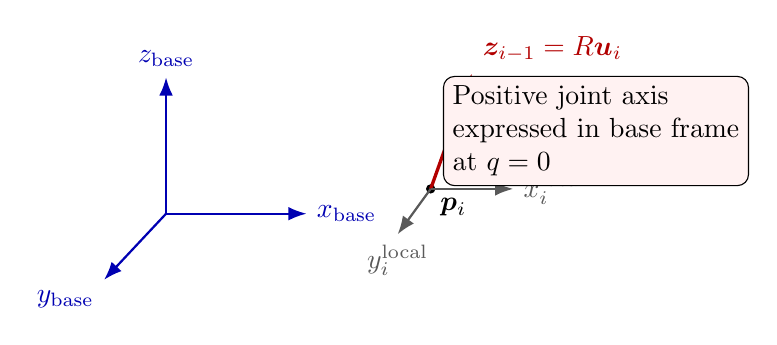
\begin{tikzpicture}[>=Latex, scale=1.05]
  \coordinate (O) at (0,0);
  \coordinate (X) at (1.7,0);
  \coordinate (Y) at (-0.75,-0.8);
  \coordinate (Z) at (0,1.65);
  \draw[->, thick, blue!70!black] (O) -- (X) node[right] {$x_{\mathrm{base}}$};
  \draw[->, thick, blue!70!black] (O) -- (Y) node[below left] {$y_{\mathrm{base}}$};
  \draw[->, thick, blue!70!black] (O) -- (Z) node[above] {$z_{\mathrm{base}}$};
  \coordinate (P) at (3.2,0.3);
  \draw[fill=black] (P) circle (1.4pt) node[below right] {$\bm{p}_i$};
  \draw[->, very thick, red!70!black] (P) -- ++(0.5,1.4) node[above right] {$\bm{z}_{i-1}=R\bm{u}_i$};
  \draw[->, thick, gray!70!black] (P) -- ++(1.0,0) node[right] {$x_i^{\mathrm{local}}$};
  \draw[->, thick, gray!70!black] (P) -- ++(-0.4,-0.55) node[below] {$y_i^{\mathrm{local}}$};
  \node[draw, rounded corners, fill=red!5, align=left] at (5.2,1.0) {Positive joint axis\\expressed in base frame\\at $q=0$};
\end{tikzpicture}
\caption{Transformation of a local URDF joint axis into the URDF base frame at the reference pose. For a revolute joint, positive $q$ follows the right-hand rule about this axis. For a prismatic joint, positive $q$ translates along this axis.}
\end{figure}

\section{Standard DH model used by PSDM}

The script uses the standard DH transform:
\begin{equation}
  {}^{i-1}\T_i = \Rot_z(\theta_i)\,\Trans_z(d_i)\,\Trans_x(a_i)\,\Rot_x(\alpha_i).
\end{equation}
Expanded as a homogeneous transform:
\begin{equation}
{}^{i-1}\T_i =
\begin{bmatrix}
\cos\theta_i & -\sin\theta_i\cos\alpha_i & \sin\theta_i\sin\alpha_i & a_i\cos\theta_i \\
\sin\theta_i & \cos\theta_i\cos\alpha_i & -\cos\theta_i\sin\alpha_i & a_i\sin\theta_i \\
0 & \sin\alpha_i & \cos\alpha_i & d_i \\
0 & 0 & 0 & 1
\end{bmatrix}.
\end{equation}

PSDM then applies the active joint coordinate through $t_i$ and $s_i$:
\begin{align}
  d_i^* &= d_i + t_i s_i q_i, \\
  \theta_i^* &= \theta_i + (1-t_i)s_i q_i.
\end{align}
In this script, $s_i=+1$ because $q_i$ is the URDF joint coordinate and the DH frames are built to use that coordinate direction.

\begin{figure}[htbp]
\centering
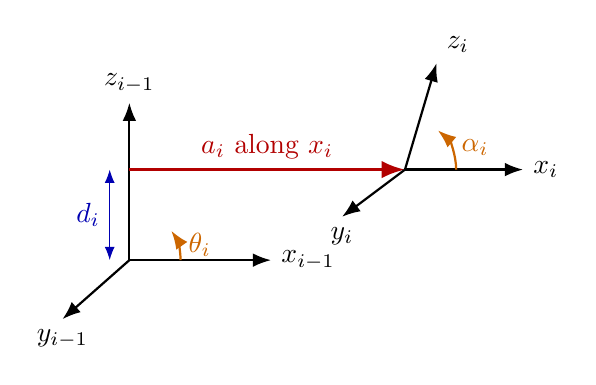
\begin{tikzpicture}[>=Latex, scale=1.0]
  \coordinate (O0) at (0,0);
  \coordinate (Z0) at (0,2.0);
  \coordinate (X0) at (1.8,0);
  \coordinate (Y0) at (-0.85,-0.75);
  \draw[->, thick] (O0) -- (Z0) node[above] {$z_{i-1}$};
  \draw[->, thick] (O0) -- (X0) node[right] {$x_{i-1}$};
  \draw[->, thick] (O0) -- (Y0) node[below] {$y_{i-1}$};
  \coordinate (P1) at (0,1.15);
  \coordinate (P2) at (3.5,1.15);
  \draw[dashed, gray] (P1) -- (P2);
  \draw[->, very thick, red!70!black] (P1) -- (P2) node[midway, above] {$a_i$ along $x_i$};
  \draw[<->, blue!70!black] (-0.25,0) -- (-0.25,1.15) node[midway,left] {$d_i$};
  \coordinate (Oi) at (3.5,1.15);
  \draw[->, thick] (Oi) -- ++(1.5,0) node[right] {$x_i$};
  \draw[->, thick] (Oi) -- ++(0.4,1.35) node[above right] {$z_i$};
  \draw[->, thick] (Oi) -- ++(-0.8,-0.6) node[below] {$y_i$};
  \draw[->, orange!80!black, thick] (0.65,0) arc[start angle=0,end angle=35,radius=0.65] node[midway,right] {$\theta_i$};
  \draw[->, orange!80!black, thick] (4.15,1.15) arc[start angle=0,end angle=50,radius=0.65] node[midway,right] {$\alpha_i$};
\end{tikzpicture}
\caption{Geometric meaning of the standard DH parameters. The implementation extracts $a_i$, $\alpha_i$, $d_i$, and $\theta_i$ from the relative transform between consecutive constructed DH frames.}
\end{figure}

\section{Mathematical construction of DH frames}

\subsection{Line representation of joint axes}

At the URDF reference pose, each active joint axis is represented as a line:
\begin{equation}
  L_i(s) = \bm{p}_i + s\bm{z}_{i-1}, \qquad s\in\R.
\end{equation}
The point $\bm{p}_i$ lies on the joint axis and $\bm{z}_{i-1}$ is the positive joint axis expressed in the URDF base frame.

\subsection{Closest points between consecutive joint axes}

For two consecutive active axes, the script finds closest points on the two infinite lines:
\begin{align}
  L_i(s) &= \bm{p}_i + s\bm{u}, \\
  L_{i+1}(t) &= \bm{p}_{i+1} + t\bm{v}.
\end{align}
Here $\bm{u}$ and $\bm{v}$ are unit vectors. Define:
\begin{equation}
  b = \bm{u}^T\bm{v}, \qquad
  \bm{w} = \bm{p}_i - \bm{p}_{i+1}, \qquad
  d = \bm{u}^T\bm{w}, \qquad
  e = \bm{v}^T\bm{w}.
\end{equation}
If the axes are not parallel, the denominator is:
\begin{equation}
  \Delta = 1-b^2.
\end{equation}
The closest-line parameters are:
\begin{align}
  s &= \frac{be-d}{\Delta}, \\
  t &= \frac{e-bd}{\Delta}.
\end{align}
The source and target closest points are:
\begin{align}
  \bm{c}_i &= \bm{p}_i + s\bm{u}, \\
  \bm{c}_{i+1} &= \bm{p}_{i+1} + t\bm{v}.
\end{align}

\begin{figure}[htbp]
\centering
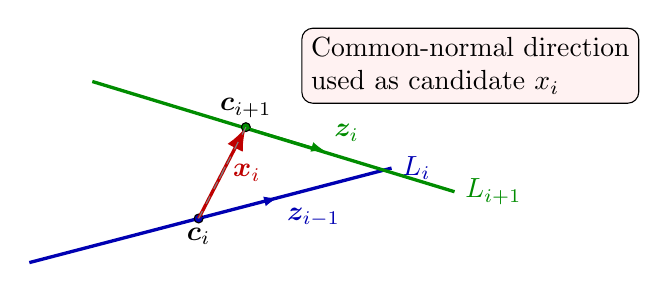
\begin{tikzpicture}[>=Latex, scale=1.0]
  \coordinate (P1) at (0.0,0.0);
  \coordinate (Q1) at (4.6,1.2);
  \coordinate (P2) at (0.8,2.3);
  \coordinate (Q2) at (5.4,0.9);
  \draw[very thick, blue!70!black] (P1) -- (Q1) node[right] {$L_i$};
  \draw[very thick, green!55!black] (P2) -- (Q2) node[right] {$L_{i+1}$};
  \coordinate (C1) at (2.15,0.56);
  \coordinate (C2) at (2.75,1.72);
  \draw[fill=blue!70!black] (C1) circle (1.6pt) node[below] {$\bm{c}_i$};
  \draw[fill=green!55!black] (C2) circle (1.6pt) node[above] {$\bm{c}_{i+1}$};
  \draw[->, very thick, red!75!black] (C1) -- (C2) node[midway, right] {$\bm{x}_i$};
  \draw[->, blue!70!black] (C1) -- ++(1.0,0.26) node[below right] {$\bm{z}_{i-1}$};
  \draw[->, green!55!black] (C2) -- ++(1.0,-0.30) node[above right] {$\bm{z}_{i}$};
  \draw[dashed, gray] (C1) -- ++(0.36,0.70);
  \draw[dashed, gray] (C2) -- ++(-0.36,-0.70);
  \node[draw, rounded corners, fill=red!5, align=left] at (5.6,2.5) {Common-normal direction\\used as candidate $x_i$};
\end{tikzpicture}
\caption{For skew axes, the common normal between closest points defines the DH $x$ direction. This is the normal case used by the script for consecutive non-parallel axes.}
\end{figure}

\subsection{Choice of $x$ axis}

The $x_i$ direction is chosen according to a simple ordered rule:
\begin{enumerate}
  \item If the closest-point separation $\bm{c}_{i+1}-\bm{c}_i$ is nonzero, set:
  \begin{equation}
    \bm{x}_i = \frac{\bm{c}_{i+1}-\bm{c}_i}{\norm{\bm{c}_{i+1}-\bm{c}_i}}.
  \end{equation}
  \item If consecutive axes intersect, use the normalized cross product when available:
  \begin{equation}
    \bm{x}_i = \frac{\bm{z}_{i-1}\times\bm{z}_i}{\norm{\bm{z}_{i-1}\times\bm{z}_i}}.
  \end{equation}
  \item If the axes are parallel or nearly parallel, reuse the previous $x$ direction projected orthogonally to the current $z$ axis, when possible.
  \item If no previous direction is available, choose an arbitrary perpendicular basis direction.
\end{enumerate}

This rule is deterministic for a given URDF and avoids adding extra dependencies. It is still a frame-construction convention, not a proof that the generated DH table is physically preferred. FK validation is the acceptance criterion.

\subsection{DH frame matrix}

Once $\bm{x}_i$ and $\bm{z}_i$ are chosen, the script constructs a right-handed frame:
\begin{align}
  \bm{y}_i &= \frac{\bm{z}_i\times\bm{x}_i}{\norm{\bm{z}_i\times\bm{x}_i}}, \\
  \bm{x}_i &\leftarrow \frac{\bm{y}_i\times\bm{z}_i}{\norm{\bm{y}_i\times\bm{z}_i}}.
\end{align}
Then:
\begin{equation}
  F_i = \begin{bmatrix}
    \bm{x}_i & \bm{y}_i & \bm{z}_i & \bm{o}_i \\
    0 & 0 & 0 & 1
  \end{bmatrix}.
\end{equation}
Here $\bm{o}_i$ is the selected origin for frame $i$.

\section{Extraction of standard DH parameters}

For each active joint $i$, the script computes the relative transform:
\begin{equation}
  {}^{i-1}\T_i = F_{i-1}^{-1}F_i =
  \begin{bmatrix}
    R & \bm{p} \\
    0 & 1
  \end{bmatrix}.
\end{equation}
The standard DH parameters are then extracted as:
\begin{align}
  \theta_i &= \atan(R_{21},R_{11}), \\
  \alpha_i &= \atan(R_{32},R_{33}), \\
  a_i &= \cos\theta_i\,p_x + \sin\theta_i\,p_y, \\
  d_i &= p_z.
\end{align}
The implementation checks that the relative transform is consistent with the standard DH form by verifying that:
\begin{equation}
  R_{31}\approx 0, \qquad -\sin\theta_i\,p_x+\cos\theta_i\,p_y\approx 0.
\end{equation}
If this check fails, the frame construction did not produce a valid standard DH relative transform and the script aborts.

\section{Residual transforms}

The generated DH frame chain is allowed to differ from the selected URDF base and tool link frames. The script therefore writes two residual transforms:
\begin{align}
  \T_{\mathrm{base}\rightarrow\mathrm{DH0}} &= F_0, \\
  \T_{\mathrm{DHn}\rightarrow\mathrm{tool}} &= F_n^{-1}\T_{\mathrm{tool}}(0).
\end{align}
The validation equation is:
\begin{equation}
  \T_{\mathrm{URDF}}(q) =
  \T_{\mathrm{base}\rightarrow\mathrm{DH0}}
  \left(\prod_{i=1}^{n} {}^{i-1}\T_i(q_i)\right)
  \T_{\mathrm{DHn}\rightarrow\mathrm{tool}}.
\end{equation}

\begin{figure}[htbp]
\centering
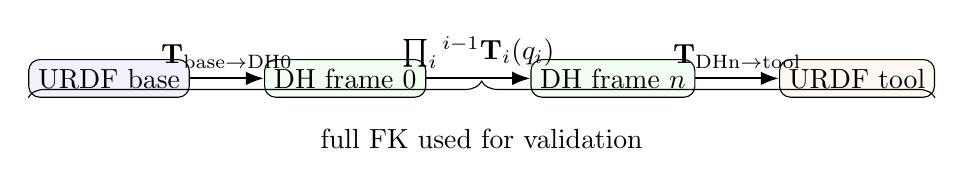
\begin{tikzpicture}[>=Latex, scale=1.0]
  \node[draw, rounded corners, fill=blue!5] (base) at (0,0) {URDF base};
  \node[draw, rounded corners, fill=green!5] (dh0) at (3,0) {DH frame 0};
  \node[draw, rounded corners, fill=green!5] (dhn) at (6.4,0) {DH frame $n$};
  \node[draw, rounded corners, fill=orange!5] (tool) at (9.5,0) {URDF tool};
  \draw[->, thick] (base) -- (dh0) node[midway, above] {$\T_{\mathrm{base}\to\mathrm{DH0}}$};
  \draw[->, thick] (dh0) -- (dhn) node[midway, above] {$\prod_i {}^{i-1}\T_i(q_i)$};
  \draw[->, thick] (dhn) -- (tool) node[midway, above] {$\T_{\mathrm{DHn}\to\mathrm{tool}}$};
  \draw[decorate, decoration={brace, amplitude=6pt}, yshift=-0.45cm] (base.south west) -- (tool.south east) node[midway, below=8pt] {full FK used for validation};
\end{tikzpicture}
\caption{Residual transforms preserve the exact relationship between the selected URDF frames and the generated DH frame chain. PSDM receives the DH table; validation and documentation retain the residual transforms.}
\end{figure}

\section{RPY normalization}

The sample URDF uses low-precision values such as \texttt{1.57} and \texttt{3.14} for nominal rotations of $\pi/2$ and $\pi$. Direct use of those literals can create artificial near-parallel or near-intersecting axes and produce large numerical DH offsets.

The script snaps each URDF RPY component to the nearest multiple of $\pi/2$ if:
\begin{equation}
  |r_{\mathrm{URDF}} - k\pi/2| \leq 10^{-2}\;\mathrm{rad}, \qquad k\in\mathbb{Z}.
\end{equation}
The same normalized transforms are used for both DH construction and URDF FK validation. The mapping report lists all joints whose RPY values were normalized.

\section{Forward-kinematics validation}

The validation process samples joint configurations and compares:
\begin{equation}
  \T_{\mathrm{URDF}}(q) \quad \text{against} \quad \T_{\mathrm{DH}}(q).
\end{equation}
For revolute joints with finite limits, the script samples uniformly in the URDF limits. Continuous joints are sampled from the configured range. Prismatic joints are sampled in their linear limits.

The position error is:
\begin{equation}
  e_p = \norm{\bm{p}_{\mathrm{URDF}} - \bm{p}_{\mathrm{DH}}}_2.
\end{equation}
The orientation error in degrees is obtained from the relative rotation:
\begin{equation}
  e_R = \cos^{-1}\left(\frac{\operatorname{tr}(R_{\mathrm{URDF}}^T R_{\mathrm{DH}})-1}{2}\right)\frac{180}{\pi}.
\end{equation}
The argument of $\cos^{-1}$ is clipped to $[-1,1]$ to avoid numerical round-off failures.

For the supplied sample, the generated validation report gave:
\begin{align}
  \max(e_p) &= 8.03\times 10^{-16}\;\mathrm{m}, \\
  \max(e_R) &= 1.71\times 10^{-6}\;\mathrm{deg}.
\end{align}

\begin{figure}[htbp]
\centering
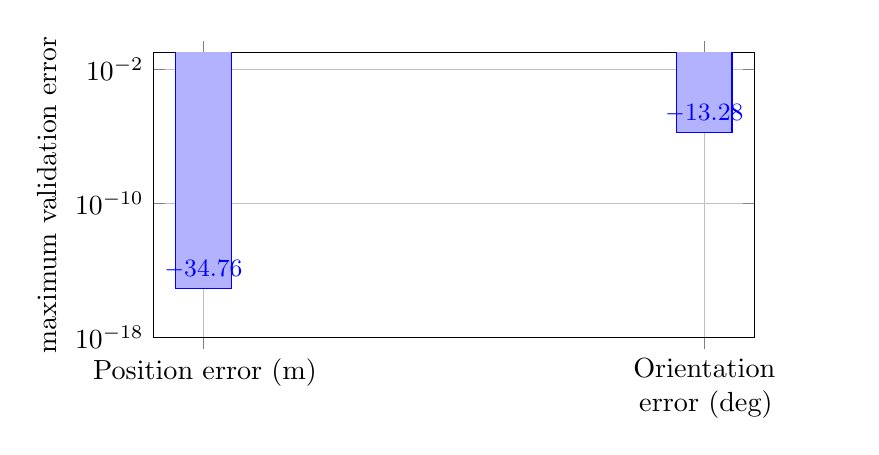
\begin{tikzpicture}
\begin{semilogyaxis}[
  width=0.76\linewidth,
  height=5.2cm,
  ybar,
  ymin=1e-18,
  ymax=1e-1,
  bar width=20pt,
  symbolic x coords={Position error (m),Orientation error (deg)},
  xtick=data,
  xticklabel style={align=center,text width=3.5cm},
  ylabel={maximum validation error},
  nodes near coords,
  every node near coord/.append style={font=\small,rotate=0,anchor=south},
  grid=both,
]
\addplot coordinates {(Position error (m),8.03e-16) (Orientation error (deg),1.71e-6)};
\end{semilogyaxis}
\end{tikzpicture}
\caption{Maximum FK validation errors reported for the supplied sample URDF and configuration. The plot uses a logarithmic vertical axis because the position and orientation errors have different units and magnitudes.}
\end{figure}

\section{Sample output DH table}

The generated sample table for \path{urdf_eb1.1.xml} and \path{urdfToDhTemplate.yaml} is shown below.

\begin{longtable}{@{}r l r r r r r r@{}}
\toprule
$i$ & Joint & $a$ (m) & $\alpha$ (rad) & $d$ (m) & $\theta$ (rad) & $t$ & $s$ \\
\midrule
1 & \path{starman_arm_joint1} & 0.0117153745 & 0 & 0 & 0 & 1 & 1 \\
2 & \path{starman_arm_joint2} & 0 & 1.5707963268 & 0.036 & 0.6947382762 & 0 & 1 \\
3 & \path{starman_arm_joint3} & 0 & 1.5707963268 & 0.797289 & 3.1415926536 & 1 & 1 \\
4 & \path{starman_arm_joint4} & 0 & 1.5707963268 & -0.161843 & 1.5707963268 & 0 & 1 \\
5 & \path{starman_arm_joint5} & 0.25 & 0 & 0.03 & -1.5707963268 & 0 & 1 \\
6 & \path{starman_arm_joint6} & 0.1199 & -1.5707963268 & -0.03 & -1.5707963268 & 0 & 1 \\
7 & \path{starman_arm_joint7} & 0 & 0 & 0 & 0 & 0 & 1 \\
\bottomrule
\end{longtable}

\section{Using the generated table in MATLAB PSDM}

The CSV file is intended for review and version control. The MAT file is directly loadable in MATLAB:
\begin{lstlisting}[language=Matlab]
load('urdf_to_dh_output/dh_table.mat', 'DH', 'joint_names');
g = [0; 0; 1];  % adjust to the PSDM base frame convention
[E, P] = PSDM.deriveModel(DH, g);
\end{lstlisting}

The gravity vector must be expressed in the PSDM base frame. If the PSDM base frame is not identical to the URDF base link frame, use the residual transform \path{T_urdf_base_to_dh_base} from \path{urdf_kinematics.json} to document and verify the intended gravity direction.

\section{Implementation map}

\begin{longtable}{@{}p{0.33\linewidth}p{0.59\linewidth}@{}}
\toprule
Function & Role \\
\midrule
\texttt{parse\_urdf} & Reads URDF joints, parent and child links, origin transforms, axes, limits, and mimic flags. \\
\texttt{get\_chain} & Walks from the configured tool link to the configured base link through parent links, then reverses the chain. \\
\texttt{urdf\_fk} & Evaluates URDF forward kinematics and records active joint axes at $q=0$. \\
\texttt{make\_dh\_frames} & Constructs DH frames from active joint axes using closest points and common normals. \\
\texttt{dh\_row} & Extracts $a$, $\alpha$, $d$, and $\theta$ from a relative standard-DH transform. \\
\texttt{dh\_fk} & Evaluates the generated DH chain, including residual transforms. \\
\texttt{validate\_fk} & Performs random-sample FK comparison and writes the validation report. \\
\texttt{write\_*} functions & Write CSV, MAT, JSON, mapping report, convention-sheet draft, and validation report. \\
\bottomrule
\end{longtable}

\section{Known limitations and acceptance criteria}

\subsection{Limitations}

\begin{enumerate}
  \item The script supports one selected serial chain only.
  \item Mimic joints are not supported.
  \item Only the coordinate policy $q_{\mathrm{PSDM}}=q_{\mathrm{URDF}}$ is implemented.
  \item The generated DH frame assignment is a deterministic convention, not a unique representation of the robot.
  \item RPY snapping is intended for URDFs that use approximate literals for exact right-angle rotations. It should be reviewed if the robot has intentional small-angle offsets near multiples of $\pi/2$.
  \item The script generates kinematic data only. It does not generate dynamic parameters, actuator constants, friction parameters, or telemetry conversion constants.
\end{enumerate}

\subsection{Acceptance criteria}

The generated DH table should be accepted only if:
\begin{enumerate}
  \item The selected base and tool link names are correct.
  \item The active joint order matches the physical and controller joint order expected by the identification workflow.
  \item The convention-sheet draft is reviewed by someone familiar with the mechanism.
  \item The FK validation report passes the configured position and orientation tolerances.
  \item The residual transforms are stored with the model artifacts.
  \item The actuator-to-joint telemetry conversion remains documented separately.
\end{enumerate}

\section{Troubleshooting}

\begin{longtable}{@{}p{0.35\linewidth}p{0.57\linewidth}@{}}
\toprule
Symptom & Likely cause and corrective action \\
\midrule
\texttt{No parent chain exists} & The configured tool link is not a link name on a descendant path from the configured base link. Check that a link name, not a joint name, is used. \\
\texttt{Mimic joint is not supported} & The selected chain contains a mimic joint. Provide an independent coordinate mapping or choose a different chain endpoint. \\
\texttt{A selected joint has a zero-length axis} & A selected active URDF joint has an invalid axis vector. Check that the chosen chain does not include nonstandard tags or malformed active joints. \\
\texttt{Internal DH frame construction failed} & The constructed consecutive frames did not satisfy the standard-DH relative transform form. Inspect the axis geometry and generated residual transforms. \\
Validation fails & Check joint order, active joint axes, base and tool links, continuous-joint sampling ranges, and whether RPY normalization is appropriate. \\
DH values are large or unstable & Check for near-parallel axes caused by low-precision URDF rotations, incorrect axis definitions, or a tool endpoint that should instead be treated as a residual fixed transform. \\
\bottomrule
\end{longtable}

\section{References}

\begin{enumerate}
  \item S. Lloyd, R. Irani, and M. Ahmadi, \emph{A numeric derivation for fast regressive modeling of manipulator dynamics}, Mechanism and Machine Theory, 2021.
  \item S. Lloyd, R. Irani, and M. Ahmadi, \emph{Application of Pseudo-Symbolic Dynamic Modeling (PSDM) in the Modeling and Calibration of a 6-DOF Articulated Robot}, preprint.
  \item PSDM MATLAB code package README.
  \item M. W. Spong and M. Vidyasagar, \emph{Robot Dynamics and Control}, referenced by the PSDM README for the DH convention.
\end{enumerate}

\appendix

\section{Minimal execution checklist}

\begin{enumerate}
  \item Install Python dependencies: \texttt{numpy}, \texttt{pyyaml}, and optionally \texttt{scipy}.
  \item Verify YAML base and tool link names.
  \item Run the script.
  \item Inspect \path{dh_mapping_report.md} and \path{conventions_sheet.draft.md}.
  \item Confirm FK validation status is \texttt{PASS}.
  \item Commit the DH table, residual transforms, configuration, and validation report with the model-generation artifacts.
\end{enumerate}

\section{Full standard DH transform for implementation checks}

For any row $[a,\alpha,d,\theta,t,s]$, the runtime coordinate substitution is:
\begin{equation}
  \theta^* = \theta + (1-t)sq, \qquad d^* = d + tsq.
\end{equation}
The evaluated transform is:
\begin{equation}
  A(q) =
\begin{bmatrix}
\cos\theta^* & -\sin\theta^*\cos\alpha & \sin\theta^*\sin\alpha & a\cos\theta^* \\
\sin\theta^* & \cos\theta^*\cos\alpha & -\cos\theta^*\sin\alpha & a\sin\theta^* \\
0 & \sin\alpha & \cos\alpha & d^* \\
0 & 0 & 0 & 1
\end{bmatrix}.
\end{equation}

\end{document}
